% \documentclass[final]{article}%
\documentclass[final, 11pt]{IEEEtran}%

% \usepackage[margin=.8in]{geometry}
\renewcommand{\baselinestretch}{1.2}

\title{Concurrent Signatures}
\ifcsname{IEEEauthorblockN}\endcsname%
  \author{\IEEEauthorblockN{Samir Benzammour}\\
    \IEEEauthorblockA{\textit{Algorithms and Complexity} \\
    \textit{RWTH Aachen University}\\
    Aachen, Germany \\
    samir.benzammour@rwth-aachen.de}
  }
\else%
  \author{Samir Benzammour\\
    \textit{Algorithms and Complexity}\\
    \textit{RWTH Aachen University}
    Aachen, Germany \\
    samir.benzammour@rwth-aachen.de
  }
\fi%
\date{\today}

% ------------------------------- packages
\usepackage{cite}
\usepackage{hyperref}
\usepackage{xcolor}
\usepackage{mathtools}
\usepackage{enumerate}
\usepackage{amsmath,stmaryrd, amssymb}
\usepackage[noabbrev]{cleveref}
\usepackage{tikz}
\usepackage{pgfplots}
\usetikzlibrary{
  calc,
  positioning,
  arrows,
  decorations.markings,
  shapes,
  fit
}
\tikzset{>=latex}
\pgfplotsset{compat=1.14}

\def\thesubsectiondis{\thesectiondis\roman{subsection}.}
\renewcommand\thesubsection{\thesection.\roman{subsection}.}

% ------------------------------- abbrevs
\newcommand{\goedel}[1]{\langle #1 \rangle}
\newcommand{\nats}{\mathbb{N}}
\newcommand{\reals}{\mathbb{R}}
\newcommand{\ints}{\mathbb{Z}}

\newcommand{\mespace}{\mathcal{M}}
\newcommand{\sspace}{\mathcal{S}}
\newcommand{\uspace}{\mathcal{U}}
\newcommand{\kspace}{\mathcal{K}}
\newcommand{\kfspace}{\mathcal{F}}

\newcommand{\Set}[1]{\ensuremath{ \{ #1 \}}}

\newtheorem{definition}{\bfseries Definition}
\newtheorem{lemma}{\bfseries Lemma}

\begin{document}
\maketitle

\begin{abstract}
  By trying to solve the problem of fair signature exchange, Chen et al. proposed a concurrent approach that works for most real applications. 
  It enables parties to produce signatures in an ambiguous way, regarding the parties identity, and are not bound by their signatures.
  They are bound to said signatures upon releasing an additional piece of information, the so-called \textit{keystone}, after which the true identity of the signer will be known.
\end{abstract}

\section{Introduction}
  \begin{frame}
	\frametitle{Introduction}
	Lorem ipsum dolor sit amet, consectetur adipisicing elit.

	\begin{itemize}
	    \item<1-> Lorem
	    \item<2-> Ipsum
	    \item<3> Dolor
	    \item<4-> Sit
	    \item<5-> Amet
	\end{itemize}
\end{frame}
  
\section{Preliminaries}
  For our following construction and the proof, later on, we will need certain constructs and tools.
These will be defined in the following.

\begin{definition}[\textnormal{\textit{Generator}}]
  Let \(\mathbb{G}\) be a cyclic group of order \(p\). Then a group generator is \(g\in\mathbb{G}\) such that it fulfills
    \[\mathbb{G} = \Set{g^i \bmod p \mid i\in\nats}\]
  This means, that by taking the generator to the multiple powers, while taking the modulus of \(p\), we can generate all elements of our given group.
\end{definition}

\begin{definition}[\textnormal{\textit{Discrete Logarithm}}]
  In a group \(\mathbb{G}\), we define the \textit{discrete logarithm} as an integer \(x\) such that \(b^x = a\) for an arbitrary integer \(a\) and \(b^x = \underbrace{b\cdot \ldots\cdot b}_{x \text{ times}}\).
\end{definition}

\begin{definition}[\textnormal{\textit{Hardness of the discrete logarithm?}}]
  \textcolor{blue}{Lorem Ipsum}
\end{definition}

\begin{definition}[\textnormal{\textit{Random Oracle}}]
  A \textit{random oracle} is a black-box algorithm which serves each \textit{unique} request with a truly random value. Moreover, it serves each duplicate request with the same answer it sent before.
\end{definition}

\begin{definition}[\textnormal{\textit{Chosen Message Attack}}]
  In a signature scheme, a \textit{chosen message attack} enables the adversary to get the signature of several messages, meaning it can query the signing oracle.
\end{definition}

\begin{definition}[\textnormal{\textit{Negligible function}}]
  We say a function \(f\) is negligible if 
  \[f(n) < \frac{1}{n^c}\]
  for a sufficiently large \(n\in\nats\). This means, that our function \(f\) converges towards 0. 
\end{definition}

\begin{definition}[\textnormal{\textit{Forking Lemma}}]
  In \cite{pcstern96} Pointcheval and Stern introduced a tool for signature schemes, the \textit{forking lemma}. 
  It states that if an algorithm \(E\) can produce a signature \(\goedel{r_1, h, r_2}\) with \(r_1\) has to be randomly chosen from a huge set, \(h\) being the hash of the message and \(r_1\), and \(r_2\) depending only on \(r_1, h\) and the message, on public input, then there exists another algorithm \(\mathcal{A}\) that controls said algorithm \(E\).
  \(\mathcal{A}\) can then replay \(E\), with replacing the signer by the simulation, to generate a second valid signature \(\goedel{r_1, h', r_2'}\) with \(h\neq h'\).
\end{definition}



\section{Construction}\label{construction}
  A signature scheme is called a \textit{concurrent signature} scheme if it holds four algorithms, namely \textbf{SETUP}, \textbf{ASIGN}, \textbf{AVERIFY}~ and \textbf{VERIFY}.
This concrete construction is based on the Schnorr signature scheme presented in \cite{schnorr1991efficient} with which we can leverage properties for our concurrent scheme.
We define our algorithms as follows
   
\subsection{\textbf{SETUP}}
  This algorithm initiates all relevant information for further course of action.
  It takes a security parameter \(\ell\) as input and, among other things, returns two large primes \(p\) and \(q\) where \(q \mid p-1\) has to hold.
  Furthermore, it returns a group generator \(g\in(\ints/p\ints)^\ast\) as well as \(\mespace, \sspace, \kspace, \kfspace\) with \(\mespace \equiv \kspace = \Set{0,1}^\ast\) and \(\sspace \equiv \kfspace = \ints_q\).
  It generates private keys \(x_i\) which are randomly chosen from \(\ints_q\), the public keys \(\Set{X_i = g^{x_i} \bmod p}\) and the set of participants \(\mathcal{U}\).
  The public keys and the set of participants are available in the public domain.
  Continuing, two cryptographic hash functions \(H_1, H_2: \Set{0,1}^\ast \to \ints_q\), alongside the function \(\textbf{KGEN} \coloneqq H_1\)
  Lastly it returns any additional parameters \(\rho\) that might be needed, and, note that, each participant keeps their respective private key \(x_i\) hidden. 

\subsection{\textbf{ASIGN}}
  This algorithm takes \(\goedel{X_i, X_j, x_i, f, M}\) as input where \(X_i, X_j\) are public keys with \(i\neq j\).
  Furthermore \(x_i\in\ints_q\) is the public key of \(i\), \(f\in\kfspace\) being the keystone-fix, which is generated through \(\textbf{KGEN}\), and \(M\in\mespace\) being the message.
  
  It calculates
    \begin{align*}
      h &= H_2(g^t X_j^f \bmod p ~\|~ M)\\
      h_1 &= h - f \bmod q\\
      s &= t - h_1 x_i \bmod q
    \end{align*}
  whereas \(t\in \ints_q\) is chosen at random.
  With this it returns a, so called, \textit{ambiguous signature} \(\sigma=\goedel{s, h_1, f}\).

\subsection{\textbf{AVERIFY}}
  This algorithm takes \(S \coloneqq \goedel{\sigma, X_i, X_j, M}\) as input, with \(\sigma=\goedel{s,h_1, f}\).
  It returns \(accept\) or \(verify\) depending on whether or not 
    \begin{equation}
      h_1 + f = H_2(g^t X_j^f \bmod p ~\|~ M) \bmod q \label{averifyeq}
    \end{equation}
  holds. 
  This equation has to hold because we have \(h_1 = h - f\) and \(h = H_2(g^t X_j^f \bmod p ~\|~ M)\).
  Therefore by rearranging it we get \autoref{averifyeq}.

\subsection{\textbf{VERIFY}}
  Lastly, this algorithm takes \(\goedel{k,S}\) as the input and checks whether or not \(\textbf{KGEN}(k) = f\), and if this is the case, checks whether or not \(\textbf{ASIGN}(S)=accept\).
  If both conditions hold, \textbf{VERIFY} returns \(accept\) and \(reject\) otherwise.
  As an overview to highlight each component, we have

  \begin{figure}[htbp]
    
    \begin{center}
      \resizebox{.99\hsize}{!}{
        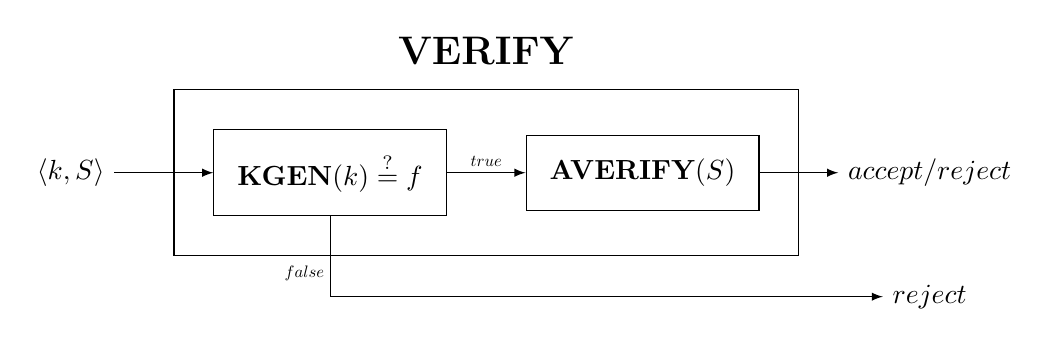
\begin{tikzpicture}[custom/.style = {rectangle, draw, align=center, inner xsep=3mm, inner ysep=3mm}, -latex]
          % nodes
          \node[custom] (kgen) {$\textbf{KGEN}(k) \overset{?}{=} f$};
          \node[custom, right=1cm of kgen.east] (averify) {$\textbf{AVERIFY}(S)$};
                \draw (kgen.east) -- node[above, scale=0.6]{$true$} (averify.west);
          \node[fit={(kgen) (averify)}, draw, outer ysep=2mm, inner xsep=5mm, inner ysep=5mm, label={\Large\textbf{VERIFY}}] (outer) {};
          
          \node[left=.75cm of outer.west] (input) {$\goedel{k,S}$};
          \node[right=1cm of averify.east] (output1) {$accept/reject$};
          \node[below=1cm of output1.south] (output2) {$reject$};
                \draw (kgen.south) |- node[left, scale=0.6, yshift=.5cm]{$false$} (output2.west);

          % connections
          \draw (input.east) to (kgen.west);
          \draw (averify.east) to (output1.west);
        \end{tikzpicture}
      }
    \end{center}
    
    \caption{\textbf{VERIFY} Components}
    \label{fig:verifycomp}
  \end{figure}


\section{Protocol}\label{protocol}
  This section is responsible for providing an understanding of the concrete signature protocol and how the algorithms defined in \autoref{construction} should be used.

We will illustrate the protocol through an exemplary interaction between a party A(lice) and B(ob). 
The following description will be visually supported through \autoref{fig:concprotocol}. 

Firstly, we start by having both parties run the \textbf{SETUP} function to initialize all necessary variables for this scheme.
Our, so called, \textit{initial signer} continues with generating a keystone \(k\in\kspace\) alongside the corresponding keystone-fix \(f\in\kfspace\).
Keep in mind, that the keystone-fix is generated through \(\textbf{KGEN}(k)\).
We set, without loss of generality, Alice as our initial signer.
Continuing, the initial signer starts off by signing a message \(M_A\in\mespace\) through \textbf{ASIGN}, while providing the private keys of herself and Bob, her own private key \(x_A\) and the keystone-fix \(f\).
Afterwards, Alice sends the resulting ambiguous signature \(\sigma_A = \goedel{s_A, h_A, f}\) to Bob.
He verifies said signature by checking if \textbf{AVERIFY} returns \(accept\), for which he additionally provides their respective public keys, as well as, Alice's message \(M_A\).
Note, that we are not trying to encrypt or obfuscate the messages in any way.
Bob and Alice, repeat the signing and verification steps analogously for Bob with the \textit{same keystone-fix}, i.e. Bob generates and sends his ambiguous signature with \(f\) and Alice verifies it.
Lastly, if Alice is satisfied with Bobs signature, she publishes the keystone \(k\) with which both \textit{ambiguous signatures} will be binding for both parties.

The power of who is generating and holding the keystone-fix is the one thing that keeps the concurrent signature scheme to be \textit{truly fair}.
Because with this, the initial signer (i.e. the one that generates the keystone(-fix)) can withhold the keystone.
However, this would not be beneficial for the withholding party in real applications.
Moreover, even if the withholding party keeps the keystone, without releasing it, the other party is not bound to the signature, meaning it is at no disadvantage. 

\begin{figure}[htbp]
  \centering
  
  \resizebox{.99\hsize}{!}{
    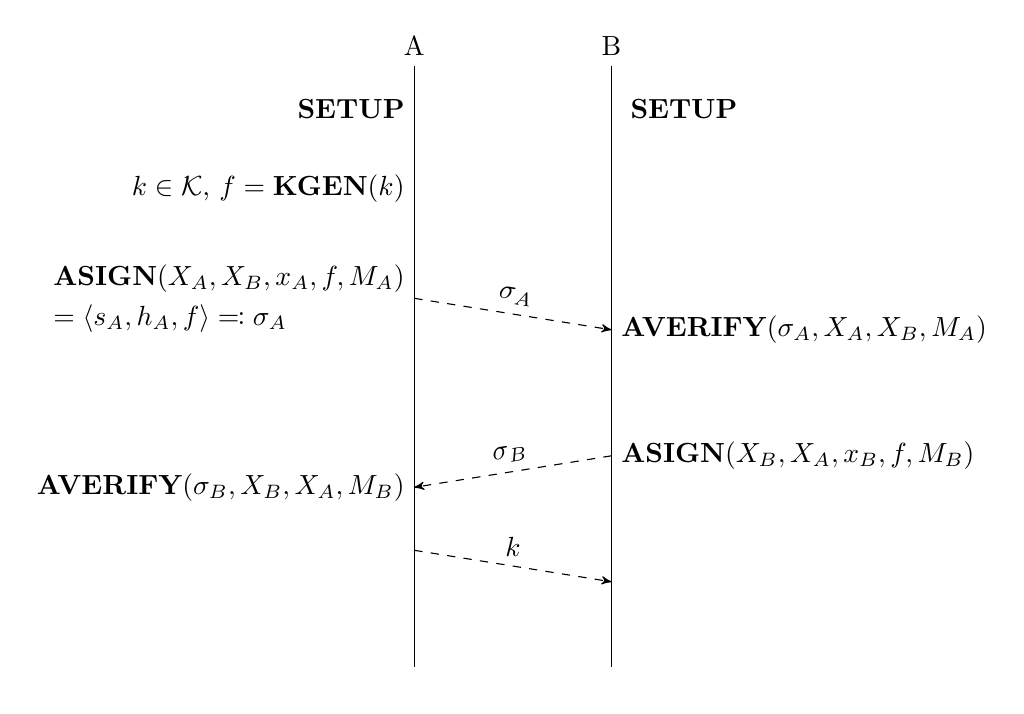
\begin{tikzpicture}[node distance=2cm,auto,>=stealth']
      \node[] (bob) {B};
      \node[left = of bob] (alice) {A};
      \node[below of=bob, node distance=8cm] (bobground) {};
      \node[below of=alice, node distance=8cm] (aliceground) {};
      
      % vertical lines
      \draw (alice) -- (aliceground);
      \draw (bob) -- (bobground);
    
      % setup
      \node[left, align=left] at ($(alice)!0.1!(aliceground)$) {\textbf{SETUP}};
      \node[right, align=right] at ($(bob)!0.1!(bobground)$) {~\textbf{SETUP}};
  
      % k keystone + KGEN
      \node[left, align=left] at ($(alice)!0.225!(aliceground)$) {$k\in\kspace$, $f = \textbf{KGEN}(k)$};
      
      % ASIGN + Arrow
      \node[left, align=left] at ($(alice)!0.4!(aliceground)$) {$\textbf{ASIGN}(X_A, X_B, x_A, f, M_A)$ \\ {$= \goedel{s_A, h_A, f} \eqqcolon \sigma_A$}};
      \draw[->, dashed] ($(alice)!0.4!(aliceground)$) -- node[sloped, above]{$\sigma_A$} ($(bob)!0.45!(bobground)$);
      
      % AVERIFY
      \node[right, align=center] at ($(bob)!0.45!(bobground)$) {$\textbf{AVERIFY}(\sigma_A, X_A, X_B, M_A)$};

      % ASIGN + Arrow
      \node[right, align=left] at ($(bob)!0.65!(bobground)$) {$\textbf{ASIGN}(X_B, X_A, x_B, f, M_B)$};
      \draw[->, dashed] ($(bob)!0.65!(bobground)$) -- node[sloped, above]{$\sigma_B$} ($(alice)!0.7!(aliceground)$);

      % AVERIFY
      \node[left, align=left] at ($(alice)!0.7!(aliceground)$) {$\textbf{AVERIFY}(\sigma_B, X_B, X_A, M_B)$};

      % keystone
      \draw[->, dashed] ($(alice)!0.8!(aliceground)$) -- node[above]{$k$} ($(bob)!0.85!(bobground)$);
    \end{tikzpicture}
  }

  \caption{Concurrent Signature Protocol - An Overview}
  \label{fig:concprotocol}
\end{figure}

\section{Security Model} \label{secmodel}
  To label our concurrent signature scheme as \textit{secure} a certain set of conditions has to hold. 
  In this scheme, we define these properties through fairness, ambiguity, and unforgeability.
  
  To define the mentioned properties we, first of all, have to define our game, in which we have an adversary \(E\) and a challenger \(C\).
  In this game \(C\) runs \textbf{SETUP} and publishes all public variables to the public domain. 
  
  The adversary can query the challenger for certain information. 
  First being a \textbf{KGen} query, meaning \(E\) can request \(C\) to generate a keystone-fix.
  It can also request \(C\) to release the keystone to a given keystone-fix through a \textbf{KReveal} query.
  The goal of \textbf{ASign} queries is to receive an \textit{ambiguous signature} from \(C\). 
  Lastly, the adversary can provide a public key for a \textbf{Private Key Extraction} query in order to receive the respective private key from \(C\).
  Note, that \(C\) does not answer to \textbf{AVerify / Verify} queries because the adversary can run the needed algorithms itself.

  \subsection{Fairness}
    In order to define fairness in our scheme, consider the previously defined game between the adversary and the challenger.
    The adversary can initially query everything it wants and \(C\) answers accordingly.
    Eventually, however, the adversary returns two public keys \(X_c, X_d\), a keystone \(k\in\kspace\), \(S=\goedel{\sigma, X_c, X_d, M}\) with \(\sigma=\goedel{s, h_1, f}\), and \(\textbf{AVERIFY}(S) = accept\).
    The adversary \(E\) wins if either
      \begin{enumerate}
        \item if \(f\) from previous query, no \textbf{KReveal} query was made on \(f\) and if \(\goedel{k,S}\) is accepted by \textbf{VERIFY}, or
        \item if \(E\) produces a second \(S' = \goedel{\sigma', X_d, X_c, M'}\) with \(\sigma' = \goedel{s', h_1', f}\) such that \(\textbf{AVERIFY}(S')=accept\).
              Continuing, \(\goedel{k,S}\) is accepted by \textbf{VERIFY}, but  \(\goedel{k,S'}\) is rejected.
      \end{enumerate}
    In the first case, the adversary produces the keystone matching to an arbitrary \(f\) which is valid.
    The second case describes the case in which the adversary is able to create a signature, with the same keystone-fix, that is not bound upon releasing the keystone.

  \subsection{Ambiguity}
    Our defined game is split into three phases now, the first query phase, the challenge phase and, lastly, the second query phase. 
    After the challenger sent all public variables to the adversary, the adversary starts the first query phase by requesting anything it wants but eventually, it has to send a, so-called, \textit{challenge tuple} to the challenger.
    This tuple is of the form \(\goedel{X_i, X_j, M}\) and represents the info the adversary wants to be challenged to.
    Then, the challenger flips a coin \(b\in\Set{0,1}\) and if \(b = 0\) it sends an ambiguous signature \(\sigma\) to the adversary on behalf of \(X_i\).
    Otherwise, the challenger sends an ambiguous signature on behalf of \(X_j\). Now, the adversary can start its second query phase, and eventually sends the challenge bit, which is a guess whose signature the challenger sent to our adversary.
    The adversary wins if the challenge bit matches the flipped coin of the challenger because then it managed to circumvent the ambiguity of the scheme.
  
    \subsection{Unforgeability}\label{unforgeability}
      We, again, consider the previously defined adversary--challenger game.
      The adversary can query everything it wants, but finally it has to return \(S=\goedel{\sigma, X_c, X_d, M}\) where \(\sigma=\goedel{s, h_1, f}\), \(X_c, X_d\) being public keys and \(M\in\mespace\) being the message.
      Continuing, the adversary wins the game if \(\textbf{AVERIFY}(S) = accept\) and if either
        \begin{enumerate}
          \item No \textbf{ASign} query was made with input \(\goedel{X_c, X_d, f, M}\) or \(\goedel{X_d, X_c, h_1, M}\).
                And no \textbf{Private Key Extraction} query was made on either \(X_c\) or \(X_d\).
          \item No \textbf{ASign} query was made with input \(\goedel{X_c, X_i, f, M}\) for all \(X_i \neq X_c, X_i\in\uspace\) and no \textbf{Private Key Extraction} query was made for \(X_c\).
        \end{enumerate}

\section{Proof of Unforgeability}\label{unforgproof}
  To start, we are going to describe the idea of the proof, which will dictate our further course of action

\begin{enumerate}[1.)]
  \item \textit{Assumption(s):} The discrete logarithm problem is hard.
  \item \textit{Proof by contraposition:} We assume our scheme is not unforgeable.
  \item We construct an algorithm that leverages the forgeability of our scheme to contradict our assumption. 
\end{enumerate}
%
If our signature scheme is \textit{not} unforgeable, there exists an algorithm \(E\) that can forge a signature with non-negligible probability.
Moreover, we define our algorithm \(\mathcal{A}\) that solves the discrete logarithm as follows:
\(\mathcal{A}\) takes \(\goedel{g,X,p,q}\) as its input and uses \(E\) as a component to solve the discrete logarithm problem, which would result in a contradiction to our assumption.

Before we start constructing our \(\mathcal{A}\) we need to show that we can rewrite our ambiguous signature format \(\sigma = \goedel{s,h_1, f}\) as \(\goedel{r_1, h, r_2}\) in order to use the forking lemma later on.
We define \(r_1\) to be \(g^t X_j^f \bmod p\), which fulfills the property that it takes its values randomly from a huge set \(\ints_q\), \(h = h_1 + f\) is the hash of the message \(M\) and \(r_1\), and lastly \(r_2 = s\) which depends solely on \(r_1, h\) and \(M\).

Furthermore, we model our hash functions \(H_1, H_2\) as random oracles, and in our following construction the algorithm \(\mathcal{A}\) simulates these random oracles and the challenger \(C\) that our forging-adversary \(E\) plays against.

Now, our algorithm \(\mathcal{A}\) starts by generating our participants \(\mathcal{U}\). It guesses that our forging-adversary \(E\) chooses \(X_\alpha\) for the position \(X_c\) in its output, and, therefore, sets \(X_\alpha = X\).
This means, that we want to acquire the discrete logarithm for the challenge public key \(X_\alpha\).
It also chooses a private key \(x_i\), which is randomly chosen from \(\ints_q\), for all participants \(i\) that are not \(\alpha\).
Otherwise, the game would be pointless due to generating the discrete logarithm, we want to acquire, on our own.
After all of that, \(\mathcal{A}\) passes on \(\goedel{g,p,q}\), as well as the public keys, to our forging-adversary.
As an overview of our setup, for now we have 

\begin{figure}[htbp]

  \begin{center}
    \resizebox{\hsize}{!}{
      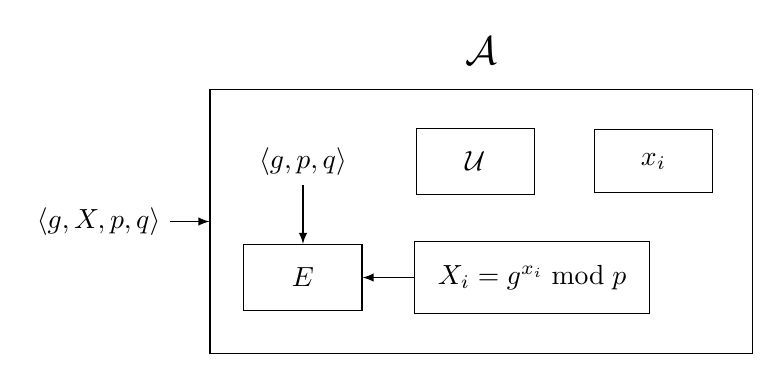
\begin{tikzpicture}[custom/.style = {rectangle, draw, align=center, minimum width=1.5cm, inner xsep=3mm, inner ysep=3mm}, -latex]
        % nodes
        \node[custom] (adversary) {$E$};
        \node[above=.75cm of adversary] (adversary_input) {$\goedel{g, p, q}$};
  
        \node[custom, right=.75cm of adversary_input] (participants) {$\mathcal{U}$};
        \node[custom, right=.75cm of participants] (priv_keys) {$x_i$};
        
        \node[custom, right=.65cm of adversary] (pub_keys) {$X_i = g^{x_i} \bmod p$};
        
        \node[fit={(adversary_input) (priv_keys) (pub_keys)}, draw, outer ysep=2mm, inner xsep=5mm, inner ysep=5mm, label={\Large$\mathcal{A}$}] (outer_box) {};
        \node[left=.5cm of outer_box.west] (input) {$\goedel{g, X, p, q}$};
        
        % connections
        \draw (input.east) to (outer_box.west);
        \draw (adversary_input.south) to (adversary.north);
        \draw (pub_keys.west) to (adversary.east);
      \end{tikzpicture}
    }
  \end{center}

  \caption{Unforgeability Proof - Overview}
  \label{fig:proofoverview}
\end{figure}

Now, our forging-adversary \(E\) can start querying requests, which include all of the queries from \autoref{secmodel} with a few additions and changes.
We add \(H_1\)- and \(H_2\) queries, with which \(E\) can query the respective oracle to acquire a hash. 
Moreover, we modify our \textbf{ASign} queries such that if \(\mathcal{A}\) receives a correct input \(\goedel{X_i, X_j, f, M}\) with \(i\neq\alpha\) we return a signature as defined in \autoref{secmodel}.
However, if \(i = \alpha\) \(\mathcal{A}\) picks random values for \(h_1\) and \(s\), and calculates the \(H_2\) hash from these values.
This happens with the premise that the random values and resulting string have never appeared in any \(H_2\) query before, otherwise \(\mathcal{A}\) chooses other values for \(h_1\) and \(s\) and starts again.

After a number of requests our forging-adversary returns an ambiguous signature \(\sigma = \goedel{s,h_1, f}\), public keys \(X_c\) and \(X_d\), and the message \(M\).
We know, from our definition in \ref{unforgeability}, that the adversary wins if \textbf{AVERIFY} accepts \(\sigma\) alongside with the public keys and the message, and if one of the following cases holds
  \begin{enumerate}
    \item No \textbf{ASign} query was made with input \(\goedel{X_c, X_d, f, M}\) or \(\goedel{X_d, X_c, h_1, M}\).
          And no \textbf{Private Key Extraction} query was made on either \(X_c\) or \(X_d\).
    \item No \textbf{ASign} query was made with input \(\goedel{X_c, X_i, f, M}\) for all \(X_i \neq X_c, X_i\in\uspace\) and no \textbf{Private Key Extraction} query was made for \(X_c\).
  \end{enumerate}

In \cite{abe20021} Abe et al. showed that our first case is negligible, assuming the hardness of the discrete logarithm problem. 
We know that our forging-adversary forges signatures with non-negligible probability, therefore, the second case must have occurred.

Furthermore, we assume that \(X_c = X_\alpha = X\) because otherwise, \(\mathcal{A}\) aborts as a result of failing to predict the correct the challenge public key.
% \textcolor{blue}{explain further?} 

Because \textbf{AVERIFY} returns \(accept\) and we know that it checks \(h_1 + f \overset{?}{=} H_2(g^s X_{c}^{h_1} X_d^f \bmod p ~\|~ M)\), we now have the equation
\[h_1 + f \overset{?}{=} H_2(g^s X_{c}^{h_1} X_d^f \bmod p ~\|~ M)\]
which leaves two new cases to investigate.

The \textit{first} case is, that \(h = h_1 + f\) has never occurred in any signature query before.
If that is the case, we rewrite our ambiguous signature to \(\goedel{r_1, h, r_2}\) and, by using the forking lemma, force \(E\) to produce a second signature \(\goedel{r_1, h', r_2'}\) with \(h\neq h'\).

Now, we have two ambiguous signatures (by rewriting the second one) with \(\sigma = \goedel{s, h_1, f}\) and \(\sigma^\prime = \goedel{s', h_1', f'}\), and \(h \neq h'\).
This results in \(h = h_1 + f \neq h_1' + f'\) which implies that either \(h_1 \neq h_1'\) or \(f \neq f'\).
The case in which \(h_1 = h_1'\) is negligible because then the relevant \(h_1\) queries would have to been calculated before the \(H_2\) queries that produced \(h\) and \(h'\) which is not possible.
In addition, it would imply that \(f = f'\) but if that would be the case the output of our \(H_1\) (that produces \(f\) and \(f'\)) oracle would have to match an \(H_2\) query.
Henceforth, we know that \(h_1 \neq h_1'\) and \(f = f'\).
As a consequence of \(h\) and \(h'\) resulting from different oracle queries we have
\begin{align}
  g^{s} X^{h_1} X_d^f &= g^{s'} X^{h_1'} X_d^{f'} \\
  s + x h_1 + f &= s' + x h_1' + f' \quad\mid f=f'\\
  s + x h_1 &= s' + x h_1' \qquad \mid h_1 \neq h_1' \label{divbyh1}\\
  x &= \frac{s-s'}{h_1' - h_1}
\end{align}
So, in the first case \(\mathcal{A}\) solves the discrete logarithm problem of \(X\) with non-negligible probability.
This contradicts the hardness of the discrete logarithm problem and therefore, for the first case, this scheme is unforgeable.

Continuing with the second case, here we assume that \(h = h'\) with \(h' = h_1' + f\) appeared in a previous signature query.
We denote said signature request with \(\goedel{X_{c'}, X_{d'}, f', M'}\) and its resulting signature with \(\sigma' = \goedel{s', h_1', f'}\).
Because we have \(h = h'\) we know that
  \[g^s X^{h_1} X_d^f \bmod p  = g^{s'} X_{c'}^{h_1'} X_{d'}^{f'} \bmod p \]
and \(M = M'\) have to hold.
Otherwise, the input of the hash functions would not be the same, and therefore \(h \neq h'\).

Here, we have to differentiate further.
If \(X_{c'} = X\), \(X_{d'} = X\) but their exponents differ, or \(X_{c'},X_{d'} \neq X\) we can easily derive the discrete logarithm \(x\) of \(X\) with the same argument as in the first case.
It is important for the case where \(X_{c'} = X\) or \(X_{d'} = X\), that the exponents differ because otherwise we would have a division by 0 in step \ref{divbyh1} of resolving to \(x\).

However, let's take a closer look at the case where \(X_{c'} = X\) or \(X_{d'} = X\), and their exponents are \textit{the same}.
If we had \(X_{c'} = X\) and \(h_1 = h_1'\), because the exponents (i.e. \(h_1, h_1'\)) are the same, then that would imply that \(f = f'\) due to \(h = h'\).
This, however, is a contradiction to the condition that no \textbf{ASign} queries can be made of the form \(\goedel{X_c, X_i, f, M}\) because we set \(X_c = X\).
Now, what if he had \(X_{d'} = X\) and \(h_1 = f'\).
Then, when \(h_1' = h' - f'\) was generated in a previous \textbf{ASign} query, \(f = h_1'\) already had to hold by definition.
Moreover, we also know that the output of \textbf{ASign} queries is determined by oracles \(H_1\) and \(H_2\).
Now, the problem is that \(f\) also is generated by \(H_1\). That means that an output of \(H_1\) has to match an \(h_1'\), that is generated by \(H_2\) and \(H_1\).
The probability of this occurring is negligible and therefore not relevant. 

With this, we showed that the discrete logarithm problem could also be solved in the second case.
Globally speaking, this means that \cref{unforgeablelemma} holds.


\section{Conclusion}\label{conclusion}
\begin{frame}
	\frametitle{Conclusion}

  \begin{center}  
    \begin{itemize}
      \setlength\itemsep{1em}
      \item sign entities without a significant disadvantage
      \item ambiguous until all parties are committed
      \item still not \textcolor{Plum}{\textit{truly fair}}
    \end{itemize}
  \end{center}
\end{frame}

\bibliography{bibliography}
\bibliographystyle{alpha}
\end{document}
